\vspace{-7pt}
\section{Design ofPCStream}
\vspace{-5pt}
We describe in detail the proposed automatic stream management technique, \textsf{\small 
PCStream}.  We first explain how we automatically extracts PCs during
run time and describe how multiple PCs are mapped to streams in an SSD.
In order to mitigate the side effect of a few outlier PCs with large lifetime variances, 
we introduce `substreams' based on a two-phase
stream assignment technique.
%{\it The PC extractor module}, which is implemented in the ... as part ... of a
%system call handler, computes a PC signature (i.e., a sum of program counter
%values) for each write-related system function. 추가 동작 설명..


Fig.~\ref{fig:architecture} shows an overall organization of \textsf{\small PCStream}.
\textit{The PC extractor module}, which is implemented in the Linux kernel as
part of a system call handler, 
computes a PC signature, which is used as a unique ID for each program context.  
We use the signature program counter~\cite{PC} as a PC signature 
by summing program counter values along the execution path to a write-related system function 
(e.g., {\tt write()}).  
With the PC signature, we can monitor the data lifetime of each write at the program context level. 
A PC signature is stored
in an inode data structure of a file system (modified for \textsf{\small PCStream})
and is delivered to \textit{the lifetime analyzer module} which estimates
expected lifetimes of data belonging to a given PC in the block device level.
In order to efficiently detect the end of data lifetime in append-only
workloads, the lifetime analyzer also intercepts TRIM~\cite{TRIM} requests. %from a file system.  %shane part
Based on the lifetime information, \textit{the PC-to-stream
mapper module} clusters PCs with similar lifetimes and maps them together to
the same stream ID.  This mapping is required because 
the number of streams in an SSD is generally less than the number of PCs in host applications.

\vspace{-10pt}
\subsection{Automatic PC computation}
%\vspace{-5pt}
As mentioned earlier, a PC is represented by a PC signature which is defined as
the sum of program counter values along the execution path of a function call that
finally reaches a write-related system function. A function call involves
pushing the next program counter, which is used as a return address, to the
stack followed by pushing a frame pointer value.  In general, by using frame
pointer values, we are able to back-track the stack frames of the process and
selectively get return addresses for generating a PC signature.  For example,
Fig.~\ref{fig:getpc}(a) shows the abstracted execution path for flushing data
in RocksDB and Fig.~\ref{fig:getpc}(b) illustrates how a PC signature is obtained
by back-tracking the stack.  
Since a frame pointer value in the stack holds the address of the previous
frame pointer, the PC extractor can easily obtain return addresses and
accumulate them to compute a PC signature. (The return addresses are pushed
before calling the \textsf{\small  write()}, \textsf{\small  BuildTable()} and \textsf{\small 
WriteLevel0Table()} functions.)

\begin{figure}[t]
	\centering
	\vspace{-7pt}
	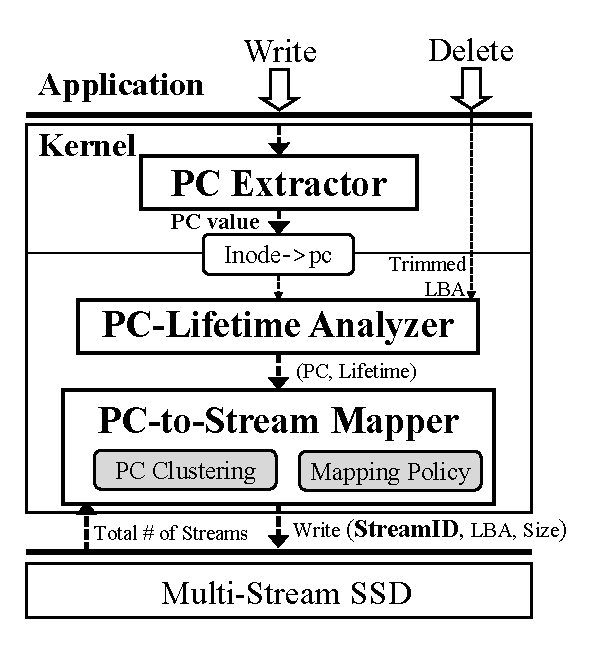
\includegraphics[width=0.6\linewidth]{figure/architecture4}
	\vspace{-10pt}
	\caption{An overall architecture of \textsf{\small PCStream}.}
	\label{fig:architecture}
	\vspace{-15pt}
\end{figure}

%The PC extractor obtains and accumulates each
%return address, which is pushed before calling the \textsf{\small  write()}, \textsf{\small 
%BuildTable()} and \textsf{\small  WriteLevel0Table()} functions, by referring the frame
%pointer which holds the address of the previous frame pointer.

%Unfortunately, C/C++ compilers often optimize an output code so
%that it does not use a frame register if possible.  
The frame pointer-based approach for computing PC signatures, however, is not
always possible because modern C/C++ compilers often do not use the frame
pointer for improving the efficiency of register allocation.
One example is a
{\tt -fomit-frame-pointer} option of GCC~\cite{GCC}. 
%While it is effective in saving
%precious resources like CPU registers, this makes it difficult for us to
%back-track return addresses only. 
Although this option allows the frame pointer to be used as a general-purpose
register for high performance, it makes very difficult for us to back-track
return addresses along the call chains.  

\begin{figure}[b]
%	\vspace{-10pt}
	\centering
	\vspace{-16pt}
	\subfloat[An abstracted execution path for flushing data.]{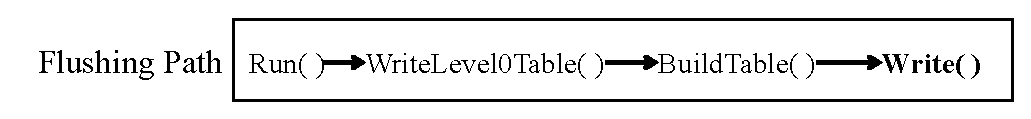
\includegraphics[width=0.45\textwidth]{figure/getpc_1}}  
	\vspace{-10pt}
	\hfill
	\subfloat[with the frame pointer.]{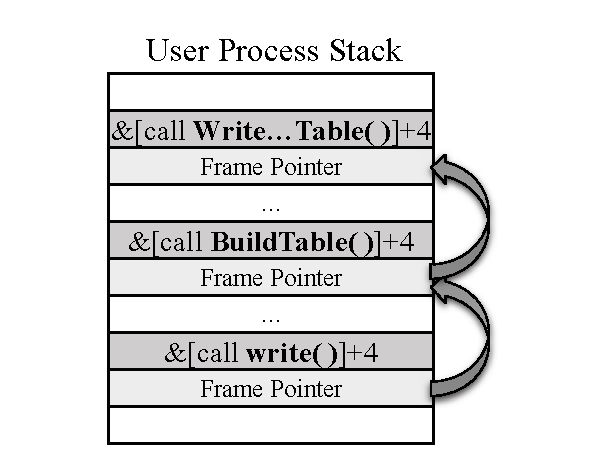
\includegraphics[width=0.245\textwidth]{figure/getpc_2}}
	\subfloat[without the frame pointer.]{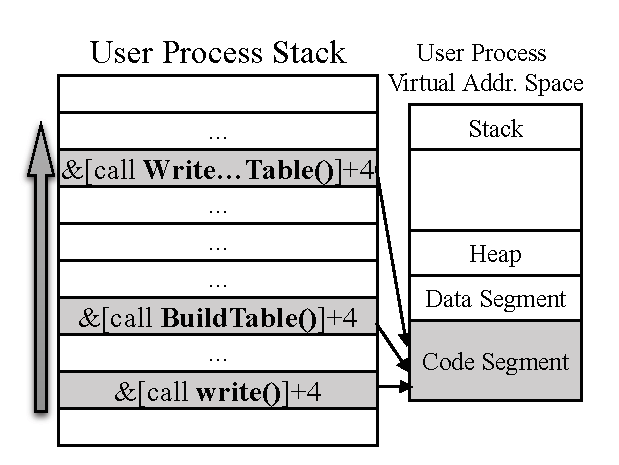
\includegraphics[width=0.25\textwidth]{figure/getpc_3}}
	\vspace{-10pt}
	%\caption{An example execution path and its PC extraction methods.}
	\caption{An example execution path and its PC extraction.} %shane part
	\label{fig:getpc}
\end{figure}

In \textsf{\small PCStream}, we employ a simple but effective workaround 
for backtracking the call stack when the frame pointer is not used.
When a write system call is made, we scan the every word in the stack and check
if it belongs to the process's code segment.  If the scanned stack word holds a
value within the address range of the code segment, we assume that it is a
return address.  Since scanning the full stack takes too long, we stop the
stack scanning procedure when a sufficient number of return address candidates
are found.  In the current version, we stop when 5 return address candidates
are found.  Although quite ad-hoc, a restricted scan is effective in
distinguishing different PCs because two different PCs
follow the same execution path up to five caller functions.   
cannot follow the same execution path to write system functions.  
(If they do, they are the same PC.) In our evaluation
with a 3.4 GHz CPU machine, the performance overhead of the restricted scan was
almost negligible, taking only 300-400 $n$sec per write system call.



\vspace{-10pt}
\subsection{PC lifetime prediction}
The prediction of PC lifetimes is rather complicated. 
The data lifetime of the append-only workload is defined 
from when a write request is issued until the TRIM command~\cite{TRIM} is issued to 
the corresponding address.
Before issuing a write request, the lifetime analyzer
maintains the written time and the address as well as the PC signature.
Upon receiving TRIM
commands destined for those LBAs, the lifetime analyzer is able to measure the
exact lifetime of those data. 
Note that, the
same PC may generate multiple data streams with different lifetimes.
We take the average lifetime as the PC's lifetime.

\vspace{-10pt}
\subsection{Mapping PCs to SSD streams}
\vspace{-5pt}
The last step inPCStream is to map
a group of PCs with similar lifetimes to an SSD stream.
This is because each SSD supports a limited number of stream IDs. For
example, SSDs used in FStream~\cite{FStream} and AutoStream~\cite{AutoStream}
support only 9 and 16 streams, respectively. To properly group multiple PCs,
the PC-to-stream mapper employs a simple 1-D clustering algorithm.  For all the
PCs, the mapper internally builds a 1-D array sorted by PCs' lifetimes.  Given
an available SSD stream number, it runs the clustering algorithm and determines
the best arrangement of PCs into different classes.  For adapting to changing
workloads, reclustering operations should be regularly performed. Since the
number of PCs created by applications is not limited, the clustering algorithm
must be efficient enough to quickly handle many PCs. Our goal in this work is
to confirm the feasibility of using PCs, so we leave
those issues as our future work.

\vspace{-10pt}
\subsection{Two-phase stream assignment}
\vspace{-5pt}

For most PCs, their lifetime distributions tend to have small variances.  
However, we observed that a few outlier PCs which have large lifetime variations. 
For example, when multiple I/O contexts are covered by the same write system function, 
the corresponding PC may represent several I/O contexts whose data lifetimes are quite different.   
Such a case occurs, for example, in the compaction module of RocksDB.
RocksDB maintains
several levels, L1, ..., L$n$, in the persistent storage, except for L0 (or a
memtable) stored in DRAM.  Once one level, say L2, becomes full, all the data
in L2 is compacted to a lower level, i.e., L3.  It involves moving data from L2
to L3, along with the deletion of the old data in L2.  In the
LSM tree~\cite{LSM}, a higher level is smaller than a lower level 
(i.e., the size of (L2) $<$ the size of (L3)). 
Thus, data stored in a higher level is invalidated more frequently than those kept
in lower levels, thereby having shorter lifetimes.

%Once the L1 becomes full,
%\textit{all} the data kept in the L1 are moved to the L2 by the compaction
%module.  The same operation is applied to the other levels (i.e., L3, ...,
%L$n-1$).  The compaction involves reading and writing data from a higher level
%(e.g., L1) to a lower level (e.g., L2).  The data in a higher level (e.g., L1)
%is then removed.  

%While the program context can be used as a useful indicator that determines the
%lifetime of data, we also observe that the same PC could generate data 
%with diverged lifetimes. One of the representative examples is the compaction
%module of RocksDB. RocksDB maintains several levels, L1, ..., L$n$, in the
%persistent storage, except for L0 (or a memtable) stored in DRAM.  Data flushed
%from the memtable are first written to the L1.  Once the L1 becomes full,
%\textit{all} the data kept in the L1 are moved to the L2 by the compaction
%module.  The same operation is applied to the other levels (i.e., L3, ...,
%L$n-1$).  The compaction involves reading and writing data from a higher level
%(e.g., L1) to a lower level (e.g., L2).  The data in a higher level (e.g., L1)
%is then removed.  In the LSM-tree, a higher level is smaller than a lower
%level. Thus, data stored in a higher level is invalidated sooner than data kept
%in lower levels, thereby having much shorter lifetimes.

Unfortunately, in the current RocksDB implementation, the compaction step is supported 
by the same execution path (i.e., the same PC) regardless of the level.
Therefore, the PC for the compaction activity cannot effectively separate data with 
short lifetimes from one with long lifetimes.
Fig.~\ref{fig:compaction}(a) shows 
the lifetime distribution collected from the compaction-activity PC.  
Since this distribution includes lifetimes of data written from all the levels, 
its variance is large.  
When we manually separate the single compaction step into several per-level compaction steps, 
as shown in Figs. 5(b) and 5(c), the lifetime distributions of per-level compaction steps 
show smaller variances.   
In particular, L2 and L3 show distinct lifetime distributions from L4.
Data from L1 are likely to have shorter lifetime, while L4 has generally
long-lived data.

\begin{figure}[!t]
\centering
\vspace{-7pt}
\hspace{2pt}
\subfloat[compaction: all levels]{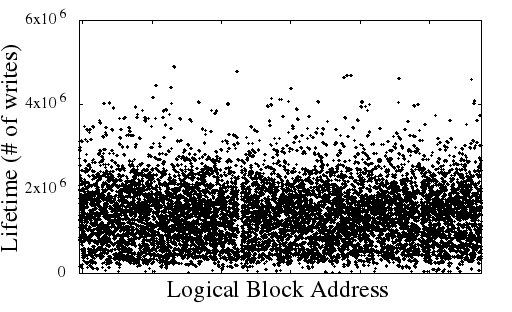
\includegraphics[width=0.23\textwidth]{figure/pc_3b}}
\subfloat[compaction: L2]{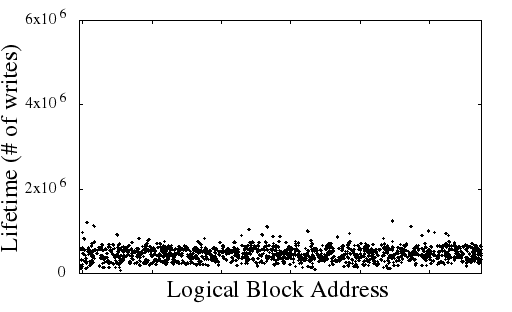
\includegraphics[width=0.23\textwidth]{figure/type_4b}}  % data from 4/03040047
\hfill
\vspace{-10pt}
\subfloat[compaction: L3]{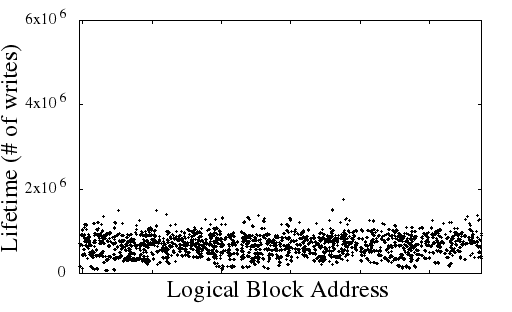
\includegraphics[width=0.23\textwidth]{figure/type_5b}}
\subfloat[compaction: L4] {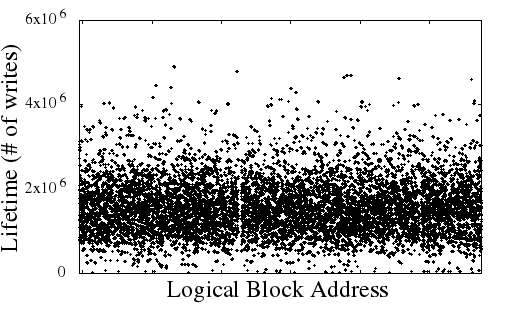
\includegraphics[width=0.23\textwidth]{figure/type_6b}}
\vspace{-5pt}
%\caption{The lifetime distribution of the compaction activity.} 
\caption{Lifetime distributions of the compaction activity at different levels.} %shane part
\label{fig:compaction}
\vspace{-15pt}
\end{figure}

In order to automatically assign data from the same PC to different SSD streams
according to their lifetimes, we devised a two-phase method that decides SSD
stream IDs both in a host level and in an SSD level.
For such a PC (e.g. the compaction-activity PC {\it pID}), \textsf{\small PCStream} assigns a
stream {\it sID} at the host level.
To separate long-lived data of 
{\it pID} (e.g., L4 data) from short-lived (future) data of {\it pID} (e.g., L1 data), 
we move the long-lived data of {\it sID} to its substream during garbage collection.   
Conceptually, a substream is used to re-separate data in the same stream so that 
future short-lived data cannot be mixed with past long-lived data in the same block.

